\documentclass[11pt]{article}
\usepackage[a4paper,margin=25mm]{geometry}
\usepackage[T1]{fontenc}
\usepackage{lmodern,microtype,amsmath,amssymb,amsthm,mathtools}
\usepackage{graphicx,booktabs,xcolor,enumitem,fancyhdr}
\usepackage[colorlinks=true,linkcolor=blue!45!black,citecolor=blue!45!black,urlcolor=blue!45!black]{hyperref}
\pagestyle{fancy}\fancyhf{}\fancyhead[L]{\small Contour quadrature with missing evaluations}\fancyhead[R]{\small Shivam Gupta}\fancyfoot[C]{\thepage}
\setlength{\headheight}{14pt}\setlength{\parskip}{3pt}
\newtheorem{theorem}{Theorem}
\newtheorem{proposition}[theorem]{Proposition}
\newcommand{\Hq}{\mathcal H_q}\newcommand{\E}{\mathcal E}
\newcommand{\one}{\boldsymbol 1}\newcommand{\norm}[1]{\left\lVert#1\right\rVert}
\title{Contour Quadrature with Missing Evaluations:\\Sharp Annular Recovery and the Cost of One Erasure}
\author{Shivam Gupta\\\small Independent Researcher\\\small\href{mailto:shivam1720406@gmail.com}{shivam1720406@gmail.com}}
\date{17 October 2026}
\begin{document}
\maketitle
\begin{abstract}
Parallel contour methods can return an incomplete set of function evaluations or shifted linear solves. How much accuracy can be recovered without completing the grid, and which missing evaluation should be retried? We study circular averages in a Laurent coefficient Hilbert space with a prescribed annular analyticity scale. For an $N$-point grid with $e$ erasures, we specialize classical optimal recovery to an FFT and an $e\times e$ precision-block solve. This gives the exact minimax error, recovered weights, and all one-step reductions in squared error in $O(N\log N+e^3)$ arithmetic and $O(N+e^2)$ storage. A closed expression shows that a single missing evaluation changes the optimal error from $\Theta(q^{N/2})$ to $\Theta(q^{N/4})$ for fixed $0<q<1$ and even $N$. A vanishing Laurent polynomial supplies an independent information lower bound. An exact four-node example shows that retry gains need not have diminishing returns. Exhaustive mask checks, rational-function experiments, and a manufactured nonnormal spectral projector validate the formulas and expose the difference between minimax protection and nominal accuracy. The method provides a conditional accuracy interface for incomplete contour computations; its assumptions and floating-point limitations are explicit.
\end{abstract}
\noindent\textbf{Keywords:} contour quadrature; optimal recovery; analytic functions; missing evaluations; spectral projectors; FFT.\\
\textbf{MSC 2020:} 65D32, 65D30, 46E22, 65F60.

\section{Introduction}
Contour integral methods transform approximation, matrix-function, and spectral problems into evaluations along a complex curve. On circular contours these evaluations are naturally parallel, but the final sum depends on a geometrically organized set of nodes. A delayed shifted solve creates a numerical question as well as a scheduling question: should the computation wait, retry, or return a reweighted result?

Suppose 63 of 64 equally spaced evaluations are available. Retaining their original weights loses exactness even for constants. Renormalizing repairs that defect but breaks cancellation of other Fourier modes. Trigonometric interpolation exploits analyticity, although clusters of missing nodes can produce very large weights. A useful recovery method should quantify what the surviving information permits and distinguish an avoidable implementation error from an unavoidable information loss.

We answer this question for Laurent series with a geometric weighted coefficient-energy bound. Positive and negative modes are allowed, accommodating functions analytic around a contour with singularities on either side. The boundary kernel is the Poisson kernel. This model permits a complete recovery calculation and an exact asymptotic result.

The main finding is that one erasure can halve the convergence exponent of the best possible recovery rule. This worst-case statement concerns the information in the surviving grid, including nonlinear postprocessing; it does not assert that every integrand suffers that loss. Arbitrary erasure effects are then expressed through a small block of the full-grid precision matrix. The same block gives retry gains without repeating a large kernel solve. We call the reference implementation \emph{ContourRepair}.

The contribution is a specialization of established optimal recovery, not a new general kernel-quadrature theory: an explicit one-erasure minimax law, complementary FFT computation on nearly complete circular grids, a nonnegative alias formula for assessing computed weights, and a retry interpretation supported by exact and numerical checks. Accurate recovery of one average does not by itself establish fault tolerance of an entire eigensolver.

\section{Relation to existing work}
Exponential periodic trapezoidal quadrature and its aliasing explanation are classical. Trefethen and Weideman~\cite{TW14}, in their treatment of unevenly spaced nodes, describe the loss of the factor-of-two advantage over trigonometric interpolation when a uniform grid is perturbed. The one-erasure result here quantifies a related phenomenon through an exact minimax error and asymptotic constant for a deleted node in a specified Laurent Hilbert ball. The general observation of reduced convergence is not new.

Optimal integration around the unit circle was studied by Chawla and Kaul~\cite{CK73}; Kress~\cite{Kress78} studied error norms and optimality of trapezoidal weights. Kernel quadrature supplies optimal weights for arbitrary nodes through a kernel system. Its Hilbert-space and Bayesian interpretations are discussed by Husz\'ar and Duvenaud~\cite{HD12}. Greedy approximation of linear functionals in reproducing kernel Hilbert spaces is analyzed by Santin, Karvonen, and Haasdonk~\cite{SKH}. These principles underlie our recovery rule and retry criterion.

Karvonen and S\"arkk\"a~\cite{KS18} exploit symmetric node sets to reduce kernel-quadrature cost. Stroud, Stein, and Lysen~\cite{SSL17} use circulant structure in inference on incomplete lattices. Here a small erasure set breaks symmetry; the reduction uses a block of the \emph{inverse} full-grid matrix. Block elimination itself is standard linear algebra. The specific spectrum, erasure loss, and contour interpretation are the objects analyzed below.

Unavailable values are an established numerical concern. Gonnet~\cite{Gonnet10} downdates explicit interpolants when adaptive integration encounters nonnumerical evaluations. We assume an analytic integrand with computationally unavailable values and calculate a deterministic, norm-conditional recovery error. Contour matrix functions~\cite{HHT08}, contour eigensolvers~\cite{SS03}, and verified contour eigenvalue calculations~\cite{IMT20} motivate the application. The last work rigorously encloses truncation and numerical errors; our floating-point code does not claim that level of verification.

Neither optimal kernel weights, FFT diagonalization, inverse-block elimination, nor general failure of exact submodularity in sequential Bayesian quadrature~\cite{HD12} is proposed as a new principle. The question is their quantitative consequence for incomplete circular contour information.

\section{Problem and analytic model}
For $0<q<1$ define the complex Hilbert space
\begin{equation}
\Hq=\left\{g(z)=\sum_{k\in\mathbb Z}a_kz^k:
\norm g_q^2:=\sum_{k\in\mathbb Z}|a_k|^2q^{-|k|}<\infty\right\}.
\label{eq:space}
\end{equation}
Cauchy--Schwarz gives locally uniform convergence on $\sqrt q<|z|<q^{-1/2}$. Values on the unit circle are continuous linear functionals. The target is
\begin{equation}
I(g)=\frac1{2\pi}\int_0^{2\pi}g(e^{i\theta})\,d\theta
=\frac1{2\pi i}\oint_{|z|=1}\frac{g(z)}z\,dz=a_0.
\label{eq:target}
\end{equation}
For $\frac1{2\pi i}\oint h(z)\,dz$, use $g(z)=zh(z)$. A periodic analytic contour parametrization can likewise absorb its derivative into $g$; the guarantees then require the corresponding Laurent norm bound.

Let $\theta_j=2\pi j/N$, $z_j=e^{i\theta_j}$, and $U=\{0,\ldots,N-1\}$. An erasure set $E\subseteq U$ leaves available nodes $A=U\setminus E$. Erasure locations are known. Initially observations $g(z_j)$, $j\in A$, are exact; bounded value errors are treated later. The theorems require no random failure model.

For $w\in\mathbb R^N$ with $w_j=0$ on $E$ set
\begin{equation}
Q_w(g)=\sum_{j\in A}w_jg(z_j),\qquad
\E(w)=\sup_{\norm g_q\le1}|I(g)-Q_w(g)|.
\label{eq:error}
\end{equation}
Optimal weights are real because the boundary kernel and target representer are real. Observations and targets can be complex.

\subsection{Meaning of the assumption}
The parameter $q$ describes an analytic scale, while $M\ge\norm g_q$ supplies an amplitude bound, yielding error $M\E(w)$. Analyticity without an amplitude bound gives no finite uniform error from finitely many values: multiply a polynomial vanishing at all observed nodes with nonzero constant term by an arbitrary scalar.

If $g$ is analytic on a larger annulus, Parseval supplies a useful sufficient bound:
\begin{equation}
\norm g_q^2\le B_-^2+B_+^2,\quad
B_\pm^2=\frac1{2\pi}\int_0^{2\pi}|g(q^{\pm1/2}e^{i\theta})|^2\,d\theta.
\label{eq:boundary}
\end{equation}
Indeed $q^k+q^{-k}\ge q^{-|k|}$. Known upper bounds on these traces suffice. Estimates inferred only from surviving values do not certify membership in the ball. Smaller $q$ imposes a stronger assumption and must not be selected solely to produce a smaller indicator.

\section{Optimal recovery and complementary computation}
The reproducing kernel on the circle is
\begin{equation}
K_q(\theta,\phi)=\sum_{k\in\mathbb Z}q^{|k|}e^{ik(\theta-\phi)}
=\frac{1-q^2}{1-2q\cos(\theta-\phi)+q^2}.
\label{eq:kernel}
\end{equation}
Write $K$ for its full-grid matrix and $C=K^{-1}$. Every principal submatrix is positive definite: zero quadratic energy would force all Fourier sums of the node coefficients to vanish, including a finite invertible Fourier system.

\begin{proposition}[Classical optimal recovery, specialized]\label{prop:optimal}
The minimum error using the available values is attained by
\begin{equation}
w_A=K_{AA}^{-1}\one_A,\quad w_E=0,\quad
\E_A^2=1-\one_A^TK_{AA}^{-1}\one_A.
\label{eq:dense}
\end{equation}
This is minimax among all algorithms using those values, including nonlinear algorithms. For $A=\varnothing$, the optimal output is zero and $\E_A=1$.
\end{proposition}
\begin{proof}
The representer of $I$ is 1. The squared residual representer norm is $1-2\one^Tw+w^TKw$. Orthogonal projection onto the span of available evaluation representers gives~\eqref{eq:dense}. Its residual $r$ vanishes at all available nodes and satisfies $\norm r_q=\E_A$ and $I(r)=\E_A^2$. Thus $\pm r/\E_A$ yield identical zero observations with targets $\pm\E_A$. Every algorithm has worst-case error at least $\E_A$; the linear rule attains it. The residual is nonzero for finite node sets, as a vanishing polynomial with nonzero constant term witnesses.
\end{proof}

The direct solve scales with the \emph{available} set. A complementary formula is preferable when few values are missing.

\begin{theorem}[Erasure formula]\label{thm:erasure}
Let $u=C\one$, $B=C_{EE}$, and $\E_U^2=1-\one^TC\one$. For nonempty $E$,
\begin{align}
w_A&=u_A-C_{AE}B^{-1}u_E,\label{eq:weights}\\
\E_A^2&=\E_U^2+u_E^TB^{-1}u_E.\label{eq:loss}
\end{align}
This includes $A=\varnothing$ by the empty-vector convention. With no erasures, $w=u$ and the added loss is zero.
\end{theorem}
\begin{proof}
Complete the square:
\[
1-2\one^Tw+w^TKw=\E_U^2+(w-u)^TK(w-u).
\]
Minimize the last term subject to $w_E=0$. Let $x=B^{-1}u_E$ and let $P_E$ embed an $E$-indexed vector into the full grid. Then $w-u=-CP_Ex$ has $E$ block $-u_E$ and $K(w-u)=-P_Ex$ has zero $A$ block. It is the constrained minimizer, with quadratic energy $x^TBx=u_E^TB^{-1}u_E$.
\end{proof}

\subsection{Spectrum and algorithmic cost}
Use $\widehat w_\ell=\sum_{j=0}^{N-1}w_je^{-2\pi i j\ell/N}$ with inverse transform scaled by $1/N$. Grouping Laurent modes modulo $N$ yields
\begin{equation}
\lambda_\ell=N\frac{q^\ell+q^{N-\ell}}{1-q^N},\quad 0\le\ell<N,
\label{eq:eigenvalues}
\end{equation}
and consequently
\begin{equation}
u_j=u_0:=\frac{1-q^N}{N(1+q^N)},\qquad
\E_U^2=\frac{2q^N}{1+q^N}.
\label{eq:full}
\end{equation}
These weights have a small shrinkage relative to $1/N$. Exactness for constants is not enforced: the constant coefficient belongs to the same bounded-energy ball.

Let $c=\operatorname{IFFT}(1/\lambda)$. Since $C_{ij}=c_{(i-j)\bmod N}$, assembling $B$ costs $O(e^2)$ after an FFT. Solve $Bx=u_E$, embed $v=P_Ex$, and compute
\begin{equation}
w=u-\operatorname{IFFT}\big(\operatorname{FFT}(v)/\lambda\big).
\label{eq:fft}
\end{equation}
The $E$ entries are zero in exact arithmetic. Weights and error cost $O(N\log N+e^3)$ arithmetic and $O(N+e^2)$ storage. Applying the rule to $d$ output components costs $O(Nd)$ more; evaluation costs are excluded.

\subsection{Nonnegative evaluation of the actual error}
The expression $1-\one_A^Tw_A$ is unsuitable for very small errors. Finite-precision weights also need not solve the normal equations exactly. Their sharp error can instead be assessed independently of optimality.
\begin{proposition}[Alias formula]\label{prop:alias}
For any real full-grid vector $w$, put $s=\sum_jw_j$ and $t=q^N$. Then
\begin{equation}
\E(w)^2=(1-s)^2+\frac{2t}{1-t}s^2+
\sum_{\ell=1}^{N-1}\frac{\lambda_\ell}{N}|\widehat w_\ell|^2.
\label{eq:alias}
\end{equation}
\end{proposition}
\begin{proof}
The coefficient representation gives
\[
\E(w)^2=|1-s|^2+\sum_{k\ne0}q^{|k|}
\left|\sum_jw_je^{ik\theta_j}\right|^2.
\]
Nonzero multiples of $N$ contribute $2ts^2/(1-t)$; the other residue classes have geometric sums $\lambda_\ell/N$. For real weights the Fourier-sign convention is immaterial after reindexing.
\end{proof}

The implementation evaluates~\eqref{eq:alias} for the stored vector and records $\max_{j\in A}|(Kw)_j-1|$. It avoids the main subtractive cancellation, but ordinary FFT arithmetic and evaluation still incur rounding. Reported values are numerical evaluations of rigorous formulas, not outward-rounded enclosures. Ill-conditioned spectra require higher precision or another representation.

\section{The exact cost of one erasure}
\begin{theorem}[One-erasure law]\label{thm:one}
Fix $0<q<1$, take $N=2m$, and erase any one node. Define
\begin{equation}
S_m(q)=\sum_{r=-m}^{m-1}\frac1{q^r+q^{-r}},\qquad
S_\infty(q)=\sum_{r\in\mathbb Z}\frac1{q^r+q^{-r}}.
\label{eq:S}
\end{equation}
The exact minimax squared error is
\begin{equation}
\E_{U\setminus\{j\}}^2=
\frac{2q^N}{1+q^N}+
\frac{(1-q^N)q^{N/2}}{(1+q^N)^2S_m(q)}.
\label{eq:one}
\end{equation}
As even $N\to\infty$,
\begin{equation}
\E_U\sim\sqrt2\,q^{N/2},\qquad
\E_{U\setminus\{j\}}\sim S_\infty(q)^{-1/2}q^{N/4}.
\label{eq:asymptotic}
\end{equation}
\end{theorem}
\begin{proof}
Circular symmetry removes dependence on $j$. Substituting $r=\ell-m$ gives
\[
C_{jj}=\frac1N\sum_{\ell=0}^{N-1}\lambda_\ell^{-1}
=\frac{(1-q^N)q^{-m}}{N^2}S_m(q).
\]
Insert this and $u_j=u_0$ into~\eqref{eq:loss}. Each summand in $S_\infty$ is at most $q^{|r|}$, so the positive bilateral series converges and $S_m\to S_\infty$. The added term is asymptotic to $q^{N/2}/S_\infty$; the full-grid term has order $q^N$. Taking square roots proves the result.
\end{proof}

\begin{figure}[tb]
\centering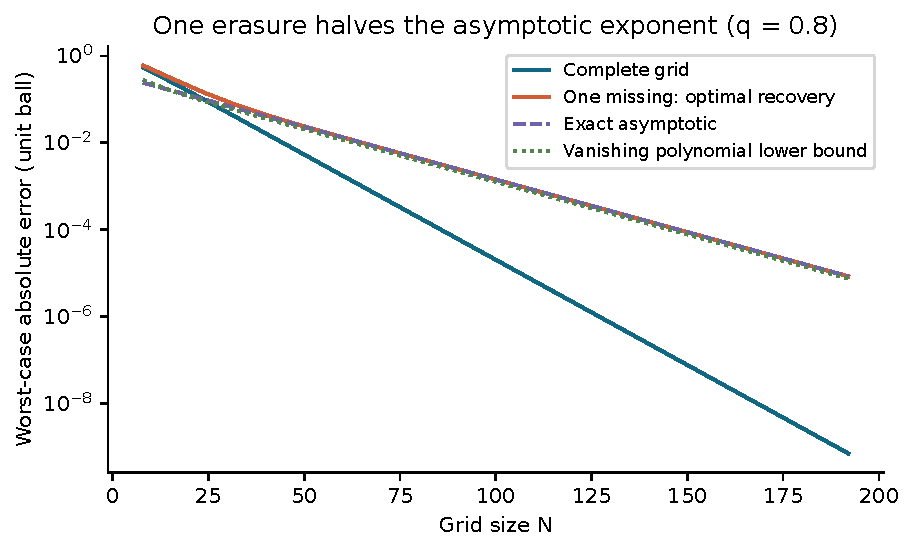
\includegraphics[width=.87\linewidth]{figures/one_erasure.pdf}
\caption{Exact minimax errors at $q=0.8$. Complete and one-erasure curves have asymptotic log slopes $\frac12\log q$ and $\frac14\log q$. The asymptotic constant and an independent polynomial lower bound are shown. These curves evaluate proved formulas, not empirical average errors.}\label{fig:one}
\end{figure}

A simple witness explains the information loss without a kernel calculation. Rotate the missing node to 1 and set
\begin{equation}
p_N(z)=z^{-(m-1)}\frac{z^{2m}-1}{z-1}
=\sum_{k=-(m-1)}^m z^k.
\label{eq:poly}
\end{equation}
It vanishes at every surviving node, has $I(p_N)=1$, and satisfies
\begin{equation}
\norm{p_N}_q^2=1+2\sum_{k=1}^{m-1}q^{-k}+q^{-m}
\sim\frac{1+q}{1-q}q^{-m}.
\label{eq:polynorm}
\end{equation}
Indistinguishable functions $\pm p_N/\norm{p_N}_q$ force error at least
$\norm{p_N}_q^{-1}\sim\sqrt{(1-q)/(1+q)}\,q^{N/4}$. This independent bound has the correct exponent but not the sharp constant.

In the asymptotic regime, compensating for one permanently unavailable value requires roughly twice as large a planned grid to match the complete-grid worst-case tolerance, with $q$ and the class fixed. This is an information comparison, not a runtime claim. Retrying the missing value can be substantially more valuable than treating it as a negligible term in a long sum.

\section{Retry gains and their limits}
\begin{proposition}[Exact one-step gain]\label{prop:gain}
For an erasure set $E$ let $B=C_{EE}$, $x=B^{-1}u_E$, and $H=B^{-1}$. Restoring $j\in E$ reduces the optimal squared error by
\begin{equation}
\Delta_j=\frac{|x_j|^2}{H_{jj}},
\label{eq:gain}
\end{equation}
where indices refer to positions within $E$.
\end{proposition}
\begin{proof}
Partition $B$ into the $j$ row and column and its complement. The block inverse formula gives
\[
u_E^TB^{-1}u_E-u_{E\setminus\{j\}}^T
B_{E\setminus\{j\},E\setminus\{j\}}^{-1}u_{E\setminus\{j\}}
=|x_j|^2/H_{jj}.
\]
The full-grid term in~\eqref{eq:loss} cancels, and $H_{jj}>0$.
\end{proof}
Computing $H$ from an $e\times e$ factorization yields all gains within the stated cost. With known retry costs $c_j>0$, $\Delta_j/c_j$ is a possible myopic priority, not an optimal multistep scheduling theorem.

\begin{proposition}[Complementarity on four nodes]\label{prop:nonmod}
Recovered information $F(A)=1-\E_A^2$ need not be submodular on equally spaced Poisson-kernel nodes. At $N=4$, $q=1/4$, set $A=\{0,2\}$, $B=\{0,2,3\}$, and $j=1$. Then
\begin{align}
F(A\cup\{j\})-F(A)&=\frac{1536}{30685}\approx0.05005703,\\
F(B\cup\{j\})-F(B)&=\frac{27744}{463885}\approx0.05980793.
\label{eq:counter}
\end{align}
The marginal gain is larger for the larger available set.
\end{proposition}
\begin{proof}
The first row of $K$ is $(5/3,15/17,3/5,15/17)$. Rational solution of the four principal systems in~\eqref{eq:dense} gives these fractions. Their difference is $76896/7886045>0$. The released program checks this with exact fractions independently of FFT recovery.
\end{proof}

General non-submodularity is already recognized in Bayesian quadrature~\cite{HD12}. This example places it explicitly inside our contour model and precludes the usual exact-submodularity greedy guarantee. Small retry budgets can be optimized exhaustively; larger scheduling problems need separate analysis.

\section{Vector outputs and inexact shifted solves}
For $g(z)=\sum a_kz^k$ with $a_k\in\mathbb C^d$, define
$\norm{g}_{q,2}^2=\sum_k\norm{a_k}_2^2q^{-|k|}$. Cauchy--Schwarz gives
\begin{equation}
\norm{I(g)-\sum_jw_jg(z_j)}_2\le M\E(w),\quad M\ge\norm{g}_{q,2}.
\label{eq:vector}
\end{equation}
Sharpness follows by placing a scalar extremizer in one output direction. For observations $\widetilde g_j=g(z_j)+\eta_j$, $\norm{\eta_j}_2\le\delta_j$,
\begin{equation}
\norm{I(g)-\sum_jw_j\widetilde g_j}_2
\le M\E(w)+\sum_j|w_j|\delta_j.
\label{eq:noise}
\end{equation}
This is an additive sufficient bound, not an exact minimax formula for the combined noisy problem. Large signed weights can amplify value error.

For a matrix $T$ without spectrum on the unit circle take
\begin{equation}
g(z)=z(zI-T)^{-1}b,\qquad I(g)=Pb,
\label{eq:projector}
\end{equation}
where $P$ is the spectral projector for eigenvalues inside the circle. Each value requires a shifted solve. If $\widetilde x_j$ has residual $r_j=b-(z_jI-T)\widetilde x_j$ and $\beta_j\ge\norm{(z_jI-T)^{-1}}_2$ is known, use $\delta_j=\beta_j\norm{r_j}_2$, since $|z_j|=1$. A small residual alone is insufficient when the resolvent norm is large.

For the manufactured validation, $T=V\Lambda V^{-1}$ is known. Set $c=V^{-1}b$, assume inner eigenvalues satisfy $|\lambda_i|<\sqrt q$ and outer ones satisfy $|\lambda_i|>q^{-1/2}$, and define
\begin{equation}
M^2:=\norm V_2^2\left[
\sum_{i\in\mathrm{in}}\frac{|c_i|^2}{1-|\lambda_i|^2/q}
+\sum_{i\in\mathrm{out}}\frac{|c_i|^2}{q|\lambda_i|^2-1}\right].
\label{eq:Mmatrix}
\end{equation}
This bounds $\norm{g}_{q,2}$: before multiplication by $V$, coefficients are diagonal geometric series; apply $\norm{Va}_2\le\norm V_2\norm a_2$ mode by mode. A known eigendecomposition validates the experiment; it is not proposed as efficient certification for an unknown production spectrum.

\section{Computational study}
All experiments below were executed with the released code. Proofs establish the theoretical claims; computations check implementation, illustrate geometry, and measure setup cost. Synthetic masks and functions do not estimate service failure rates or a population of engineering problems.

\subsection{Protocol and independent checks}
The environment was Python 3.9.6, NumPy 1.26.4, SciPy 1.13.1, and Matplotlib 3.9.4 on an Apple M4 Pro with 24 GB memory. BLAS and OpenMP thread counts were set to one; the exact command, seeds, and platform information are recorded in the repository.

For all $2^8=256$ erasure masks at $N=8$, $q=0.7$, the FFT rule is compared with an independently assembled dense Poisson-kernel solve. Every retry gain is checked by explicitly restoring its node and recomputing the error. Other tests compare the alias formula to a direct 799-mode Laurent sum, construct a unit-norm residual extremizer attaining the bound, test a noisy three-component output, and reject invalid input and excessive spectral conditioning. The four-node example uses exact fractions.

One-erasure calculations use $q=0.8$ and $N=8,16,\ldots,192$. FFT errors agree with~\eqref{eq:one} within relative squared-error tolerance $10^{-7}$. Figure~\ref{fig:one} shows the exact formula, asymptotic constant, and polynomial bound. Exact-arithmetic asymptotics extend beyond the plot; the double-precision code limits the full-grid condition number to $10^{12}$.

\subsection{Geometry and baselines}
Four baselines use identical available values: equal renormalized weights, periodic nonuniform trapezoidal weights from angular gaps, Fourier least squares of degree at most eight, and largest symmetric Fourier degree $d=\lfloor(|A|-1)/2\rfloor$. Fourier weights are the constant-coefficient pseudoinverse row with relative singular-value cutoff $10^{-12}$. These do not cover all regularized interpolation strategies. The dense kernel solve is a correctness and timing comparator producing the same rule as recovery.

At $N=64$, $q=0.8$, take $e=1,2,4,8,12,16$. Missing nodes form a consecutive block, a dispersed set $\{\lfloor kN/e\rfloor:0\le k<e\}$, or 100 uniformly sampled subsets per count. Five errors and weight $\ell^1$ norms are recorded per mask, giving 3,060 method--mask records. Figure~\ref{fig:geometry} and Table~\ref{tab:geometry} show the geometry effect.

\begin{figure}[tb]
\centering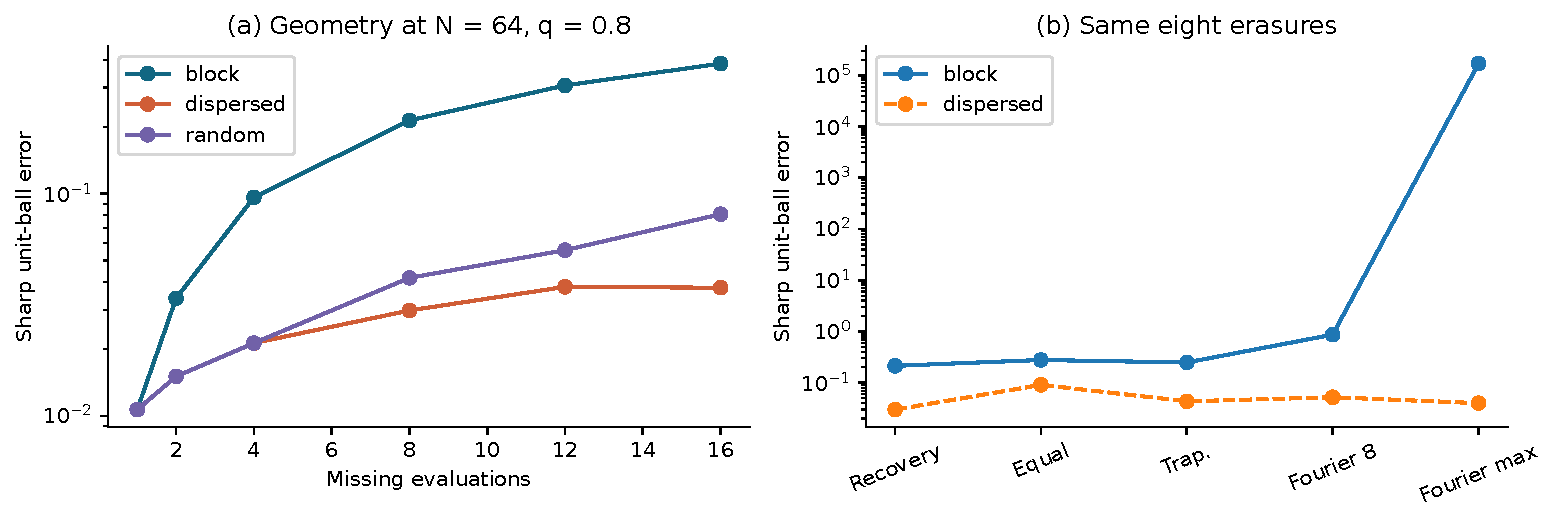
\includegraphics[width=\linewidth]{figures/geometry.pdf}
\caption{Left: optimal error for block, dispersed, and random erasures; the random curve is a median over 100 masks per count. Right: five rules with the same eight erased evaluations. All quantities are sharp unit-ball errors. Nearly maximal-degree Fourier reconstruction is unstable for the block mask.}\label{fig:geometry}
\end{figure}
\begin{table}[tb]\centering
\caption{Sharp unit-ball errors for eight erasures, $N=64$, $q=0.8$.}\label{tab:geometry}
\begin{tabular}{lrr}\toprule
Rule & Block & Dispersed\\\midrule
ContourRepair / dense optimum & 0.213314 & 0.029810\\
Equal renormalization & 0.277477 & 0.090717\\
Nonuniform trapezoid & 0.247966 & 0.043273\\
Fourier degree 8 & 0.866065 & 0.052025\\
Fourier maximal degree & $1.69031\times10^5$ & 0.039822\\\bottomrule
\end{tabular}
\end{table}

The block optimum is about 7.16 times the dispersed optimum for eight erasures. Recovery minimizes worst-case error by construction; the experiment quantifies the geometric dependence. On the block, Fourier-maximal weights have $\ell^1$ norm about $2.83\times10^6$, compared with 1.0684 for recovery. Equation~\eqref{eq:noise} makes this stability difference consequential.

\subsection{Rational functions: minimax versus nominal accuracy}
Forty rational functions have three inner poles with radii sampled in $[0.25,0.72]$, three outer poles in $[1.4,2.2]$, independent uniform phases, and complex Gaussian residues and constants. Each is normalized by its analytic $\Hq$ norm. The reference is its exact constant Laurent coefficient. Each is evaluated on the same grid with block, dispersed, and random eight-erasure masks: 120 function--mask cases and 600 method records. Block and dispersed masks rotate by case index; random masks are sampled independently.

\begin{table}[tb]\centering
\caption{Median absolute errors across 40 unit-norm rational functions per pattern. Nominal and worst-case errors are different objectives.}\label{tab:rational}
\begin{tabular}{lrrr}\toprule
Rule & Block & Dispersed & Random\\\midrule
ContourRepair & $4.63\times10^{-2}$ & $3.99\times10^{-4}$ & $9.33\times10^{-4}$\\
Equal & $9.20\times10^{-2}$ & $2.10\times10^{-3}$ & $2.88\times10^{-2}$\\
Nonuniform trapezoid & $1.60\times10^{-2}$ & $5.58\times10^{-4}$ & $6.83\times10^{-4}$\\
Fourier degree 8 & $1.11\times10^{-2}$ & $6.52\times10^{-5}$ & $4.81\times10^{-4}$\\
Fourier maximal degree & 1.14 & $3.46\times10^{-7}$ & $2.38\times10^{-6}$\\\bottomrule
\end{tabular}
\end{table}
All 600 errors are within their norm bounds. Recovery improves on equal weighting but does not generally minimize nominal error on this smoother family. Fourier maximal degree is especially accurate on dispersed masks and unreliable on a block. Recovery minimizes sensitivity over the entire stated ball; interpolation can be preferable when stronger information is justified. The results do not establish uniform empirical superiority.

\subsection{A nonnormal spectral projector}
The $48\times48$ test matrix has 16 equally spaced eigenvalues of radius 0.65 and 32 of radius 1.6. Its real eigenvector matrix has two independent orthogonal factors and singular values geometrically spaced from 1 to 10, so $\kappa_2(V)=10$; the complex matrix is generally nonnormal. A Gaussian $b$ defines the action. The independent reference is $V_{\mathrm{in}}(V^{-1}b)_{\mathrm{in}}$. Contour values use dense shifted solves, not diagonal evaluation.

At $q=0.8$, \eqref{eq:Mmatrix} gives $M=35.9279$. For block, dispersed, and random masks, recovery relative errors are $8.88\times10^{-2}$, $1.00\times10^{-3}$, and $2.67\times10^{-3}$. Absolute errors 0.6185, 0.006995, and 0.01862 are below bounds 7.664, 1.071, and 1.395. All 15 method--mask errors obey their bounds, which are conservative here. Fourier maximal degree is more accurate on the dispersed mask; its relative error exceeds 9 on the block. This is a manufactured projector-action test, not an evaluation of FEAST or a verified eigenvalue count.

\subsection{Retry selection and setup cost}
For $E=\{0,1,\ldots,7,16,24,40,56\}$ at $N=64$, $q=0.8$, largest-gain selection first restores node 4. Error falls from 0.21437 to 0.11402; the median of 100 random first retries is 0.18773. Figure~\ref{fig:retry} shows the greedy path, random-order quantiles, and exhaustive optima for budgets zero through four. At budget two, greedy gives 0.07229 whereas the optimum is 0.05623, directly demonstrating the limitation of myopic selection.

\begin{figure}[tb]
\centering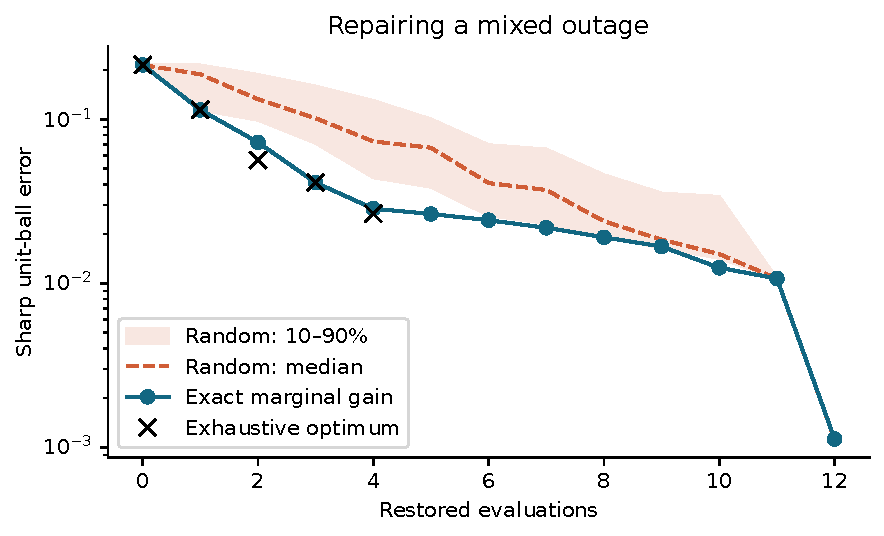
\includegraphics[width=.84\linewidth]{figures/retries.pdf}
\caption{Repairing twelve erasures. Exact one-step gains improve on the median random order in early steps of this instance, but greedy selection is not globally optimal. The two-retry optimum is below the greedy result. Shading shows empirical 10--90\% quantiles over 100 random orders.}\label{fig:retry}
\end{figure}

For timing, eight random nodes are erased for grid sizes from 64 to 1024, doubling at each step, and $q=\exp(-12/N)$ keeps conditioning comparable. This changes the class with $N$ and is not a fixed-class convergence experiment. After one warmup, seven calls are timed per method. FFT setup includes error and retry diagnostics; the dense comparator constructs and solves the available kernel system. Weight differences are below $8\times10^{-16}$.
\begin{table}[tb]\centering
\caption{Local setup medians over seven repeats, eight erasures, $q=\exp(-12/N)$. Function evaluations and shifted solves are excluded.}\label{tab:timing}
\begin{tabular}{rrrr}\toprule
$N$ & FFT (ms) & Dense (ms) & Dense / FFT\\\midrule
64 & 0.0563 & 0.0361 & 0.64\\
128 & 0.0567 & 0.1202 & 2.12\\
256 & 0.0714 & 0.5613 & 7.86\\
512 & 0.1191 & 2.9615 & 24.86\\
1024 & 0.1878 & 18.3903 & 97.93\\\bottomrule
\end{tabular}
\end{table}

Dense setup wins at the smallest size. The roughly 98-fold setup ratio at $N=1024$ is not an end-to-end solver speedup. The advantage matters when outputs reuse a grid or many outage patterns are assessed, and only if setup is material relative to evaluation costs. Figure~\ref{fig:timing} displays the measured scaling.

\begin{figure}[tb]
\centering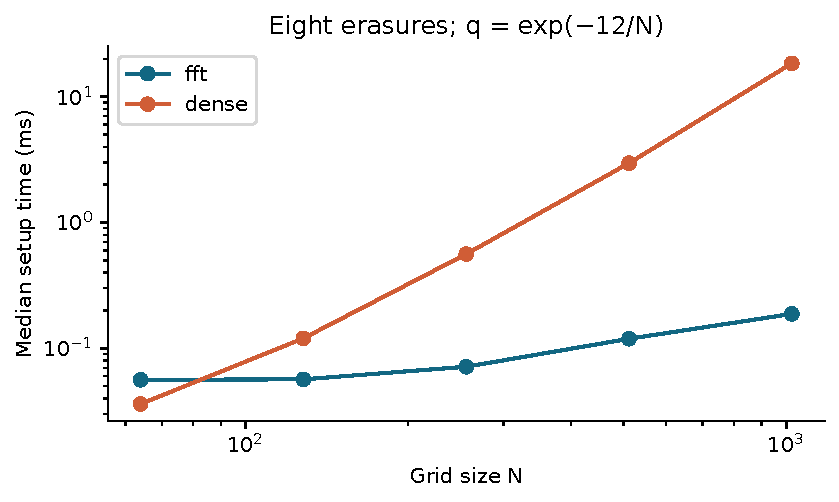
\includegraphics[width=.77\linewidth]{figures/timing.pdf}
\caption{Setup time versus grid size for eight erasures. The changing $q=\exp(-12/N)$ holds conditioning comparable. Each point is a median of seven local calls; the FFT routine includes error and retry diagnostics. No evaluation or shifted-solve runtime is included.}\label{fig:timing}
\end{figure}

\section{Practical use and limitations}
A computational service could expose three outputs after incomplete evaluation: the recovered integral, its model-conditional error budget, and the marginal value of each retry. Potential settings include repeated frequency-response studies, spectral filtering, and simulations paying for remote solves. The measurable product hypothesis is reduced avoidable waiting or retries while meeting a tolerance. The experiments establish no customer-demand, financial-return, patentability, or production-reliability claim.

The guarantee requires a defensible $q$, amplitude bound $M$, and, for inexact solves, value-error or resolvent bounds. Poles approaching the circle narrow the admissible annulus. Eigenvalues alone do not control nonnormal resolvent growth. Large $N$ at fixed $q$ makes the kernel poorly conditioned despite exact-arithmetic validity. The code rejects spectra beyond its condition limit; interval or multiple-precision implementations would be needed for rigorous numerical enclosures.

The experiments cover synthetic rational functions, one manufactured matrix, and local timing. They do not test large sparse PDE models, nonlinear eigenproblems, distributed runtimes, or failure-dependent sampling bias. Nominal results favor Fourier rules on some smoother functions. A practical solver should compare stability-aware Fourier reconstruction when stronger assumptions are justified.

An asymmetric Laurent norm could describe different interior and exterior singularity distances. Its full-grid kernel remains Fourier diagonal, but its one-erasure asymptotics need analysis. Direct optimization of the combined approximation and bounded-noise error could reduce amplification with clustered erasures. Retry selection should also incorporate joint gains, costs, and completion-time distributions. The counterexample and greedy gap prevent an unqualified greedy guarantee.

\section{Conclusion}
Missing contour evaluations change the available analytic information. In a geometric Laurent Hilbert ball, one missing node halves the optimal exponential convergence rate, while arbitrary erasures admit complementary precision-block computation. The FFT algorithm reproduces dense optimal recovery and exposes error, weight sensitivity, and one-step retry gains. It provides a bounded, reproducible basis for deciding when incomplete contour information suffices and when an additional evaluation is necessary.

\section*{Code and reproducibility}
Source, tests, experiment definitions, raw tables, figures, and manuscript source are at \url{https://github.com/shi1720/contour-repair}. Code is under the MIT license; environment and fixed seeds are recorded. Run \texttt{python3 -m unittest discover -s tests -v}, then \texttt{python3 run\_experiments.py} with the stated thread limits. Checked bound violations cause experiment failure.

\appendix
\section{Analytic norm of the rational benchmarks}
For
\[
g(z)=c_0+\sum_i\frac{r_i}{z-p_i}+\sum_j\frac{s_j}{z-t_j},
\quad |p_i|<\sqrt q,\quad |t_j|>q^{-1/2},
\]
the constant coefficient is $a_0=c_0-\sum_js_j/t_j$. Geometric expansions give
\begin{equation}
\norm g_q^2=|a_0|^2+
\sum_{i,i'}\frac{r_i\overline r_{i'}}{q-p_i\overline p_{i'}}+
\sum_{j,j'}\frac{s_j\overline s_{j'}}{t_j\overline t_{j'}(qt_j\overline t_{j'}-1)}.
\label{eq:rationalnorm}
\end{equation}
Double sums are real in exact arithmetic. There is no finite Fourier truncation in the normalization or target. This calculation is independent of the recovery kernel.

\section{Reference algorithm}
For $N,q,E$, the code performs:
\begin{enumerate}[leftmargin=*,itemsep=2pt]
\item Form~\eqref{eq:eigenvalues}; check positivity and conditioning.
\item Set $u_0=1/\lambda_0$ and compute $c=\operatorname{IFFT}(1/\lambda)$.
\item Assemble $B_{ab}=c_{(E_a-E_b)\bmod N}$ and solve $Bx=u_0\one$.
\item Embed $x$ and evaluate~\eqref{eq:fft}; set erased entries exactly to zero.
\item Evaluate stored-vector error using~\eqref{eq:alias} and record the normal-equation residual on available nodes.
\item Solve for $B^{-1}$ and compute gains~\eqref{eq:gain}. Add the value-error term only with valid $\delta_j$.
\end{enumerate}
No $N\times N$ matrix is stored. All-erased and no-erased cases are handled; repeated and out-of-range indices are rejected. The dense baseline uses a stable sine-squared kernel expression without the inverse-block identity.

\begin{thebibliography}{99}
\bibitem{CK73} M. M. Chawla and V. Kaul, Optimal rules for numerical integration round the unit circle, \emph{BIT Numerical Mathematics}, 13 (1973), 145--152. \href{https://doi.org/10.1007/BF01933486}{doi:10.1007/BF01933486}.
\bibitem{Kress78} R. Kress, On error norms of the trapezoidal rule, \emph{SIAM Journal on Numerical Analysis}, 15 (1978), 433--443. \href{https://doi.org/10.1137/0715027}{doi:10.1137/0715027}.
\bibitem{TW14} L. N. Trefethen and J. A. C. Weideman, The exponentially convergent trapezoidal rule, \emph{SIAM Review}, 56 (2014), 385--458. \href{https://doi.org/10.1137/130932132}{doi:10.1137/130932132}.
\bibitem{HD12} F. Husz\'ar and D. Duvenaud, Optimally-weighted herding is Bayesian quadrature, in \emph{Proceedings of UAI 2012}, 377--386. \url{https://auai.org/uai2012/papers/213.pdf}.
\bibitem{KS18} T. Karvonen and S. S\"arkk\"a, Fully symmetric kernel quadrature, \emph{SIAM Journal on Scientific Computing}, 40 (2018), A697--A720. \href{https://doi.org/10.1137/17M1121779}{doi:10.1137/17M1121779}.
\bibitem{SKH} G. Santin, T. Karvonen, and B. Haasdonk, Sampling based approximation of linear functionals in reproducing kernel Hilbert spaces, \emph{BIT Numerical Mathematics}, 62 (2022), 279--310. \href{https://doi.org/10.1007/s10543-021-00870-3}{doi:10.1007/s10543-021-00870-3}.
\bibitem{SSL17} J. R. Stroud, M. L. Stein, and S. Lysen, Bayesian and maximum likelihood estimation for Gaussian processes on an incomplete lattice, \emph{Journal of Computational and Graphical Statistics}, 26 (2017), 108--120. \href{https://doi.org/10.1080/10618600.2016.1152970}{doi:10.1080/10618600.2016.1152970}.
\bibitem{Gonnet10} P. Gonnet, Increasing the reliability of adaptive quadrature using explicit interpolants, \emph{ACM Transactions on Mathematical Software}, 37 (2010), Article 26, 1--32. \href{https://doi.org/10.1145/1824801.1824804}{doi:10.1145/1824801.1824804}.
\bibitem{HHT08} N. Hale, N. J. Higham, and L. N. Trefethen, Computing $A^\alpha$, $\log(A)$, and related matrix functions by contour integrals, \emph{SIAM Journal on Numerical Analysis}, 46 (2008), 2505--2523. \href{https://doi.org/10.1137/070700607}{doi:10.1137/070700607}.
\bibitem{SS03} T. Sakurai and H. Sugiura, A projection method for generalized eigenvalue problems using numerical integration, \emph{Journal of Computational and Applied Mathematics}, 159 (2003), 119--128. \href{https://doi.org/10.1016/S0377-0427(03)00565-X}{doi:10.1016/S0377-0427(03)00565-X}.
\bibitem{IMT20} A. Imakura, K. Morikuni, and A. Takayasu, Verified partial eigenvalue computations using contour integrals for Hermitian generalized eigenproblems, \emph{Journal of Computational and Applied Mathematics}, 369 (2020), 112543. \href{https://doi.org/10.1016/j.cam.2019.112543}{doi:10.1016/j.cam.2019.112543}.
\end{thebibliography}
\end{document}
